%%%%%%%%%%%%%%%%%%%%%%%%%%%%%%%%%%%%%%%%%%%%%%%%%%%%%%%%%%%%%%%%
%%                                                            %%
%%   essentialsOfLatin, Italian translation 2017              %%
%%                                                            %%
%% From:  Henry C. Pearson, Essentials Of Latin For Beginners %%
%%        (1915, New York, American Book Company)             %%
%%                                                            %%
%%    https://archive.org/details/essentialslatin04peargoog   %%
%%                                                            %%
%% Translated by g.p.ciceri <gp.ciceri@gmail.com>             %%
%% ---------------------------------------------------------- %%
%% This translation is Licensed under                         %%
%% Creative Commons Attribution-ShareAlike 4.0 International  %%
%% https://creativecommons.org/licenses/by-sa/4.0/            %%
%%                                                            %%
%%%%%%%%%%%%%%%%%%%%%%%%%%%%%%%%%%%%%%%%%%%%%%%%%%%%%%%%%%%%%%%%

% āēīōū
% ăĕĭŏŭ




\documentclass[nols]{tufte-handout}

%\geometry{showframe} % display margins for debugging page layout

\usepackage{fontspec}
\usepackage{ifxetex}
\setmainfont[Path=./fonts/palatino-linotype/, ItalicFont=palai.ttf, BoldFont=palab.ttf]{pala.ttf}


% \defaultfontfeatures{Mapping=tex-text}
% \setromanfont[Path=./fonts/TeX-Gyre-Schola/,Mapping=tex-text]{TeX Gyre Schola}
% \setsansfont[Path=./fonts/TeX-Gyre-Heros/,Scale=MatchLowercase,Mapping=tex-text]{TeX Gyre Heros}
% \setmonofont[Path=./fonts/TeX-Gyre-Cursor/,Scale=MatchLowercase]{TeX Gyre Cursor}

\usepackage{lipsum}
\usepackage{url}
\usepackage{longtable}
\usepackage{stackengine}

\usepackage{graphicx} % allow embedded images
  \setkeys{Gin}{width=\linewidth,totalheight=\textheight,keepaspectratio}
  \graphicspath{{graphics/}} % set of paths to search for images
\usepackage{amsmath}  % extended mathematics
\usepackage{booktabs} % book-quality tables
\usepackage{units}    % non-stacked fractions and better unit spacing
\usepackage{multicol} % multiple column layout facilities
\usepackage{lipsum}   % filler text
\usepackage{fancyvrb} % extended verbatim environments
  \fvset{fontsize=\normalsize}% default font size for fancy-verbatim environments

% Standardize command font styles and environments
\newcommand{\doccmd}[1]{\texttt{\textbackslash#1}}% command name -- adds backslash automatically
\newcommand{\docopt}[1]{\ensuremath{\langle}\textrm{\textit{#1}}\ensuremath{\rangle}}% optional command argument
\newcommand{\docarg}[1]{\textrm{\textit{#1}}}% (required) command argument
\newcommand{\docenv}[1]{\textsf{#1}}% environment name
\newcommand{\docpkg}[1]{\texttt{#1}}% package name
\newcommand{\doccls}[1]{\texttt{#1}}% document class name
\newcommand{\docclsopt}[1]{\texttt{#1}}% document class option name
\newenvironment{docspec}{\begin{quote}\noindent}{\end{quote}}% command specification environment

% concetti morfosintattici
\usepackage{xspace} 
\newcommand{\noun}{\textsc{sostantivo}\xspace}
\newcommand{\nouns}{\textsc{sostantivi}\xspace}
\newcommand{\adject}{\textsc{aggettivo}\xspace}
\newcommand{\adjects}{\textsc{aggettivi}\xspace}
\newcommand{\gnumber}{\textsc{numero}\xspace}
\newcommand{\gnumbers}{\textsc{numeri}\xspace}
\newcommand{\gender}{\textsc{genere}\xspace}
\newcommand{\genders}{\textsc{generi}\xspace}
\newcommand{\gcase}{\textsc{caso}\xspace}
\newcommand{\gcases}{\textsc{casi}\xspace}
\newcommand{\tense}{\textsc{tempo}\xspace}
\newcommand{\mood}{\textsc{modo}\xspace}
\newcommand{\gverb}{\textsc{verbo}\xspace}
\newcommand{\gverbs}{\textsc{verbi}\xspace}
\newcommand{\adjective}{\textsc{aggettivo}\xspace}
\newcommand{\nom}{\textsc{nom}\xspace}
\newcommand{\gen}{\textsc{gen}\xspace}
\newcommand{\dat}{\textsc{dat}\xspace}
\newcommand{\acc}{\textsc{acc}\xspace}
\newcommand{\voc}{\textsc{voc}\xspace}
\newcommand{\abl}{\textsc{abl}\xspace}
\newcommand{\gexit}{\textsc{uscita}\xspace}
\newcommand{\gexits}{\textsc{uscite}\xspace}
\newcommand{\declinazione}{\textsc{declinazione}\xspace}
\newcommand{\masc}{\textsc{maschile}\xspace}
\newcommand{\femm}{\textsc{femminile}\xspace}
\newcommand{\neut}{\textsc{neutro}\xspace}

\newcommand{\indic}{\textsc{indicativo}\xspace}
\newcommand{\imper}{\textsc{imperativo}\xspace}
\newcommand{\gcong}{\textsc{congiuntivo}\xspace}
\newcommand{\ott}{\textsc{ottativo}\xspace}
\newcommand{\partic}{\textsc{participio}\xspace}
\newcommand{\infin}{\textsc{infinito}\xspace}

\newcommand{\pres}{\textsc{presente}\xspace}
\newcommand{\imperf}{\textsc{imperfetto}\xspace}
\newcommand{\aor}{\textsc{aoristo}\xspace}
\newcommand{\fut}{\textsc{futuro}\xspace}
\newcommand{\perf}{\textsc{perfetto}\xspace}
\newcommand{\pperf}{\textsc{piuccheperfetto}\xspace}

\newcommand{\sing}{\textsc{singolare}\xspace}
\newcommand{\plur}{\textsc{plurale}\xspace}
\newcommand{\dual}{\textsc{duale}\xspace}

\newcommand{\si}{\textsc{sing}\xspace}
\newcommand{\pl}{\textsc{plur}\xspace}
\newcommand{\du}{\textsc{dual}\xspace}

\newcommand{\att}{\textsc{attivo}\xspace}
\newcommand{\med}{\textsc{medio}\xspace}
\newcommand{\pass}{\textsc{passivo}\xspace}
\newcommand{\medpass}{\textsc{medio-passivo}\xspace}


% italianitudini
\renewcommand{\figurename}{Figura}
\renewcommand{\tablename}{Tabella}
\renewcommand{\contentsname}{Indice}

% fix per un qualche problema
\ifxetex
  \newcommand{\textls}[2][5]{%
    \begingroup\addfontfeatures{LetterSpace=#1}#2\endgroup
  }
  \renewcommand{\allcapsspacing}[1]{\textls[15]{#1}}
  \renewcommand{\smallcapsspacing}[1]{\textls[10]{#1}}
  \renewcommand{\allcaps}[1]{\textls[15]{\MakeTextUppercase{#1}}}
  \renewcommand{\smallcaps}[1]{\smallcapsspacing{\scshape\MakeTextLowercase{#1}}}
  \renewcommand{\textsc}[1]{\smallcapsspacing{\textsmallcaps{#1}}}
\fi

% too many float...
\extrafloats{100}
% āēīōū
% ăĕĭŏŭ

\title{Essentials Of Latin. Elementi di Latino. \newline Lezione II - Prima Declinazione, temi in -ā- (continua).}

\author[gpciceri]{a cura di Milagathòs: Milo's help to enjoy humanities.}

\date{22 Gennajo 2017} % without \date command, current date is supplied


\begin{document}

\hyphenation{co-niu-ga-zio-ne}

\maketitle% this prints the handout title, author, and date

\begin{marginfigure}[-2.5cm]
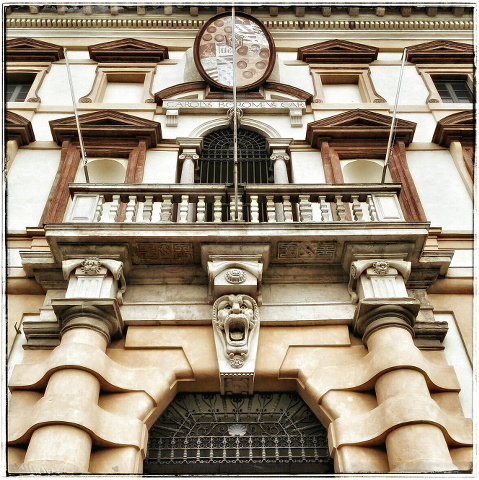
\includegraphics{smallthumb-lesson_I.jpeg}
\setfloatalignment{b}
\end{marginfigure}


\begin{abstract}
\noindent
Queste lezioni riprendono il testo introduttivo al Latino di Pearson\cite{pearson1915}, del quale seguono la numerazione; la struttura di ogni lezione è piuttosto regolare: inizia con \textsc{cenni di morfologia e di sintassi latina}, seguita da un \textsc{piccolo vocabolario} per il lessico; ci sono infine vari \textsc{esercizi} di traduzione e di composizione latina.

\bigskip
\noindent
Lezione II - Prima Declinazione, temi in -ā-, aggettivi femminili e maschili, vocabolario, esercizi.
\end{abstract}

%\printclassoptions
% āēīōū
% ăĕĭŏŭ

\newthought{32.} Gli aggettivi femminili della Prima Declinazione sono declinati come i nomi.
\begin{center}
\textbf{rosa pulchra}, f., \textit{la rosa bella} \\
radice \textbf{rosā- pulchrā-} \quad tema \textbf{ros- pulchr-}
\end{center}

\begin{fullwidth}
\begin{table}[!htbp]
  \centering
  \begin{tabular}{l l}
    %\toprule
	& \multicolumn{1}{c}{\textsc{Singolare}}\\

    \nom & ros\textbf{a} pulchr\textbf{a}, \textit{la rosa bella} (soggetto) \\
    \gen & ros\textbf{ae} pulchr\textbf{ae}, \textit{della rosa bella} \\
    \dat & ros\textbf{ae} pulchr\textbf{ae}, \textit{alla rosa bella}  \\
    \acc & ros\textbf{am} pulchr\textbf{am}, \textit{la rosa bella} (compl.oggetto) \\
    \voc & ros\textbf{a} pulchr\textbf{a}, \textit{o rosa bella} \\
    \abl & ros\textbf{ā} pulchr\textbf{ā}, \textit{per mezzo della rosa bella} \\
	
	\multicolumn{2}{c}{\textemdash} \\
	& \multicolumn{1}{c}{\textsc{Plurale}}\\

	\nom & ros\textbf{ae} pulchr\textbf{ae}, \textit{le rose belle} (soggetto)  \\
    \gen & ros\textbf{ārum} pulchr\textbf{ārum}, \textit{delle rose belle}   \\
    \dat & ros\textbf{īs} pulchr\textbf{īs}, \textit{alle rose belle} \\
    \acc & ros\textbf{ās} pulchr\textbf{ās}, \textit{le rose belle} (compl.oggetto)  \\
    \voc & ros\textbf{ae} pulchr\textbf{ae}, \textit{o rose belle}  \\
    \abl & ros\textbf{īs} pulchr\textbf{īs}, \textit{per mezzo delle rose belle} \\

    %\bottomrule
  \end{tabular}
  %\caption[bottom]{Prima Declinazione. \textbf{stella, -ae}, f.}
  \label{tab:normaltab}
  %\zsavepos{pos:normaltab}
\end{table}
\end{fullwidth}

\newthought{Osservazioni.} L'aggettivo e il nome sono \textit{nello stesso caso}, l'aggettivo non precede o segue sempre il nome: la posizione delle parole in Latino è piuttosto libera (vedi nel seguito (82.)).

\newthought{33. Frasi Modello.} Esamina le seguenti frasi:
 
\begin{itemize}
\item[\textsc{1.}] \textbf{Rosa pulchra est}, \textit{la rosa è bella}.  
\item[\textsc{2.}] \textbf{Rosae pulchra sunt}, \textit{le rose sono bella}.    
\end{itemize}
In queste frasi \\
\begin{itemize}
\item[\textsc{a.}] I soggetti \textbf{(rosa, rosae)} sono in caso nominativo. 
\item[\textsc{b.}] Il verbo è al singolare quando il soggetto è singolare; quando il soggetto è plurale, il verbo è al plurale.  
\item[\textsc{c.}] Gli aggettivi al predicato nominale \textbf{(pulchra, pulchrae)} concordano con il soggetto in caso, genere e numero.  
\end{itemize}

\newthought{34. Regole di Sintassi}
\begin{itemize}
\item[\textsc{1. Il caso del Soggetto.}] Il soggetto di un verbo in modo finito è sempre al nominativo.  
\item[\textsc{2. Concordanza del predicato.}] Un predicato (nominale) costituito da un aggettivo concorda con la parola a cui si riferisce in \textit{caso, genere e numero}. Un predicato (nominale) costituito da un nome concorda solo nel caso con la parola a cui si riferisce. 
\end{itemize}

\newthought{35. Vocabolario}

\begin{multicols}{2}
    \noindent \hangindent=1em \textbf{fabula, -ae}, f., \textit{favola}.  \\
    \noindent \hangindent=1em \textbf{sagitta, -ae}, f., \textit{freccia}.  \\
	\noindent \hangindent=1em \textbf{insula, -ae}, f., \textit{isola}.  \\
	\noindent \hangindent=1em \textbf{terra, -ae}, f., \textit{terra, regione}.  \\
	
	\noindent \hangindent=1em \textbf{bona, -ae}, agg.f. \textit{buona}.  \\
	\noindent \hangindent=1em \textbf{lata, -ae}, agg.f. \textit{larga, ampia}.  \\
	\noindent \hangindent=1em \textbf{longa, -ae}, agg.f. \textit{lunga}.  \\
	\noindent \hangindent=1em \textbf{magna, -ae}, agg.f. \textit{grande}.  \\
	\noindent \hangindent=1em \textbf{pulchra, -ae}, agg.f. \textit{bella}.  \\
	
	\noindent \hangindent=1em \textbf{est}, v. \textit{(egli, ella, esso) è, c'è}.  \\
	\noindent \hangindent=1em \textbf{sunt}, v. \textit{(loro, essi) sono, ci sono}.  \\
	
	\noindent \hangindent=1em \textbf{ubi}, avv. \textit{dove, quando}.  \\
	\noindent \hangindent=1em \textbf{non}, avv. \textit{non}.  \\
	\noindent \hangindent=1em \textbf{et}, cong. \textit{e}.  \\
	
\end{multicols}
% āēīōū
% ăĕĭŏŭ

\newthought{36. Esercizi}
\\
\textsc{I.} \quad
\textsc{1.}~Fabulae longae sunt. \quad
\textsc{2.}~Terra est lata et pulchra. \quad
\textsc{3.}~Ubi est pulchra insula? \quad
\textsc{4.}~Luna est pulchra. \quad
\textsc{5.}~Bonae sagittae sunt longae. \quad
\textsc{6.}~Non est pulchra. \quad
\textsc{7.}~Magnae sunt insulae. \quad
\textsc{8.}~Latis terris. \quad
\textsc{9.}~Luna et stellae sunt pulchrae. \quad
\textsc{10.}~Via est lata. \quad
\textsc{11.}~Ubi sunt insulae magnae? \quad
\textsc{12.}~Sagittarum longarum. \quad
\textsc{13.}~Vias silvarum. 
\\
\textsc{II.} \quad
\textsc{1.}~La regina è bella. \quad
\textsc{2.}~È una grande isola. \quad
\textsc{3.}~Dove sono le lunghe frecce? \quad
\textsc{4.}~Sono belle ragazze. \quad
\textsc{5.}~La regione non è ampia. \quad
\textsc{6.}~È una buona storia.

\begin{figure}[!b]
  %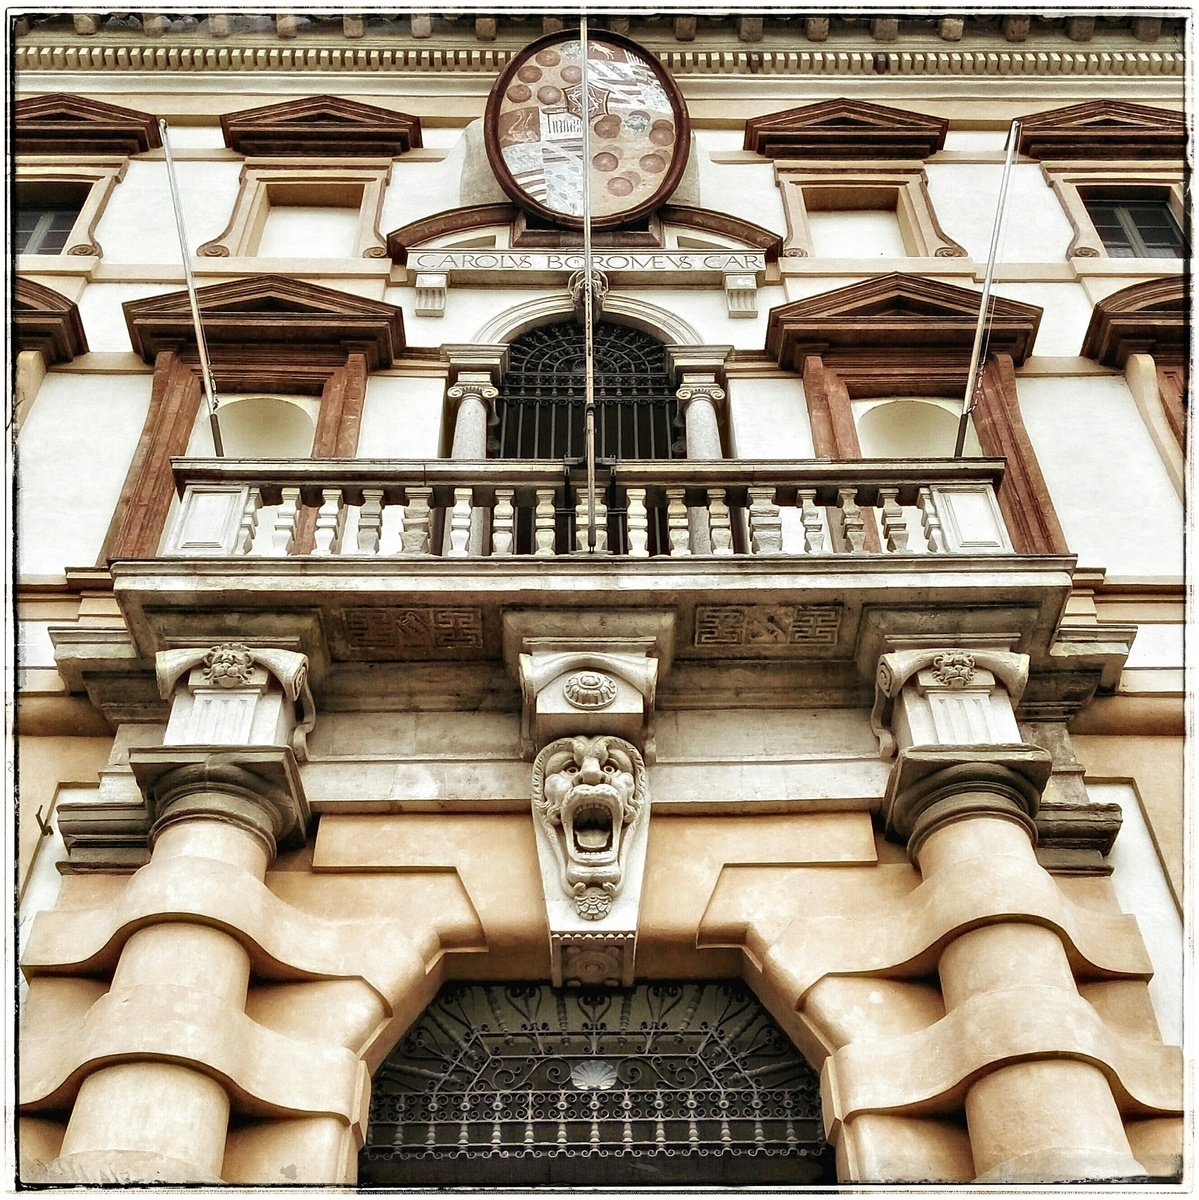
\includegraphics{thumb-lesson_I.jpeg}
  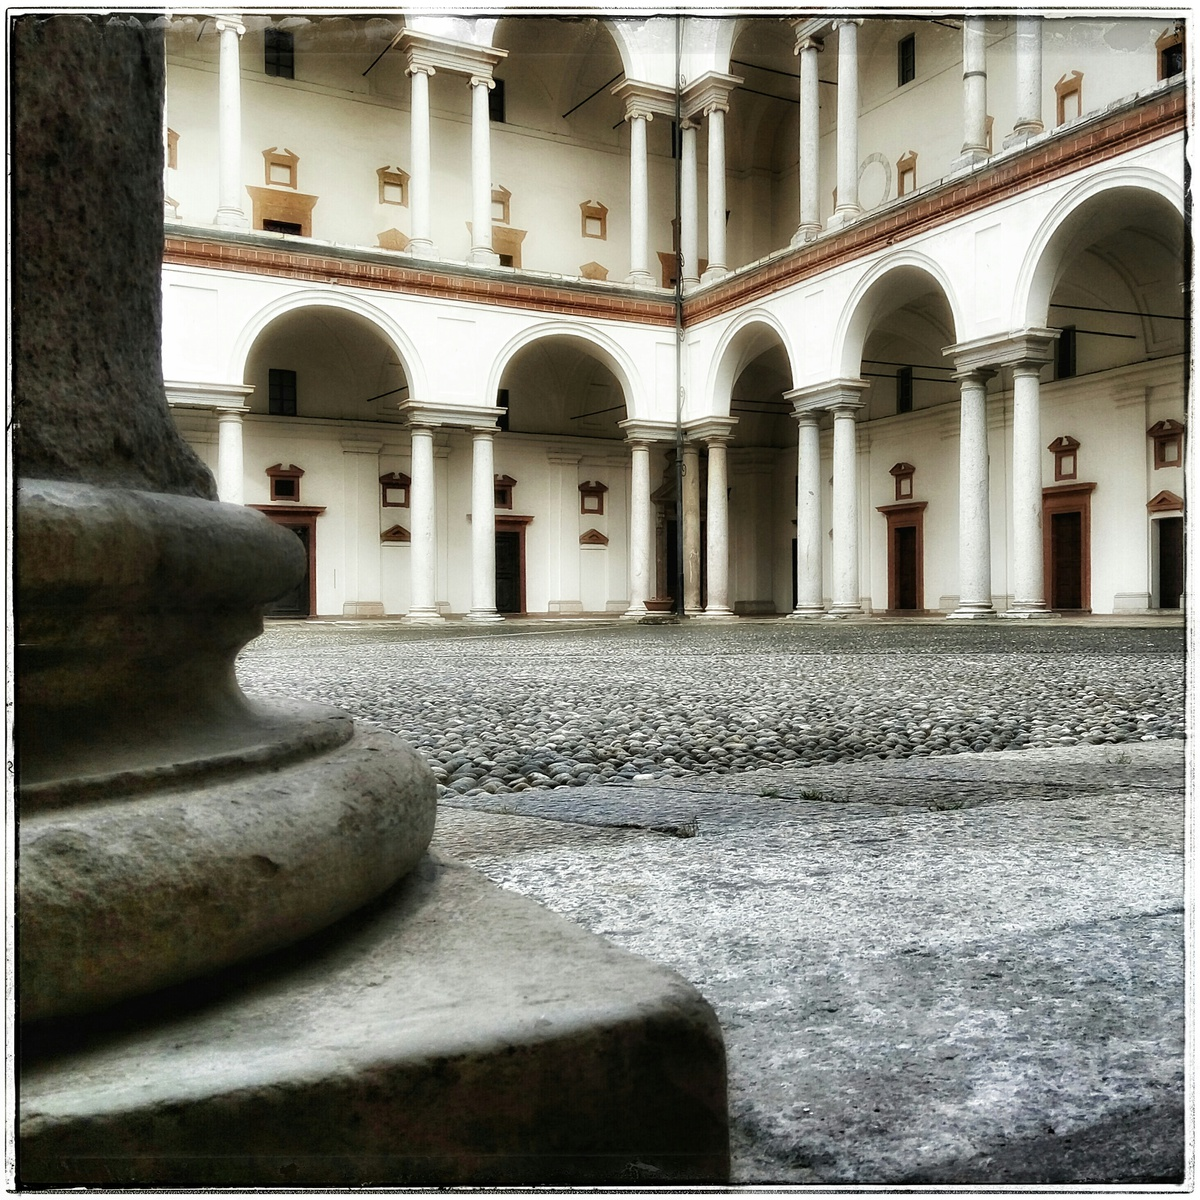
\includegraphics[width=0.8\linewidth]{thumb-lesson_II.jpeg}
  %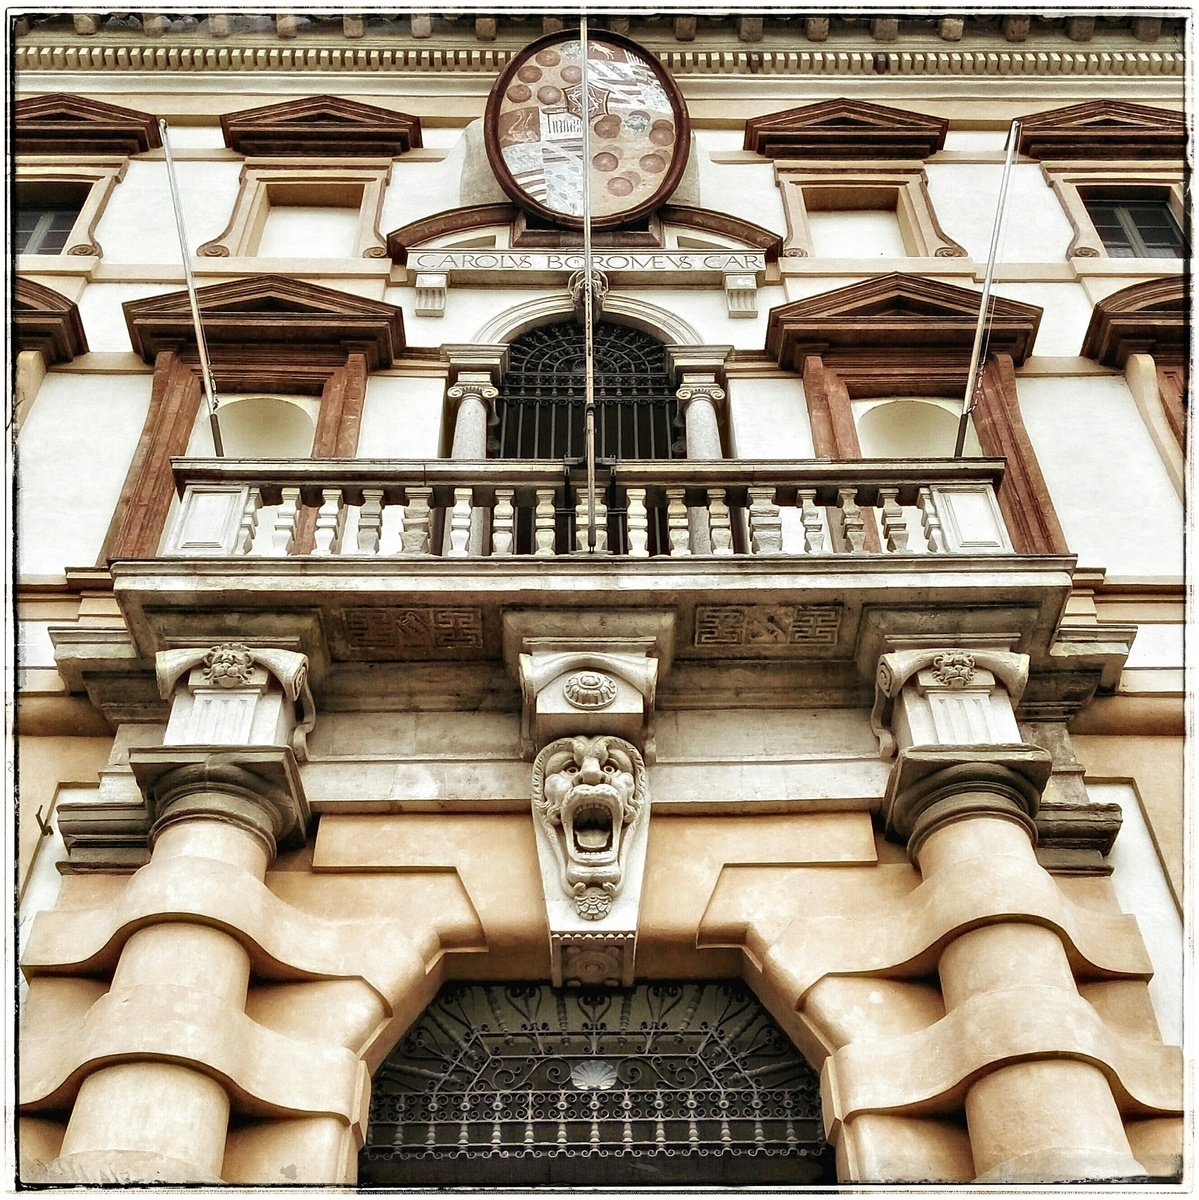
\includegraphics{thumb-lesson_I.jpeg}
  \caption{Pavia: Almo Collegio Borromeo}
  \label{fig:textfig}
  %\zsavepos{pos:textfig}
  %\setfloatalignment{b}
\end{figure}

 

\nobibliography{latinBiblio}
\bibliographystyle{alpha}


\end{document}
